\documentclass[10pt,]{article}
\usepackage{lmodern}
\usepackage{amssymb,amsmath}
\usepackage{ifxetex,ifluatex}
\usepackage{fixltx2e} % provides \textsubscript
\ifnum 0\ifxetex 1\fi\ifluatex 1\fi=0 % if pdftex
  \usepackage[T1]{fontenc}
  \usepackage[utf8]{inputenc}
\else % if luatex or xelatex
  \ifxetex
    \usepackage{mathspec}
  \else
    \usepackage{fontspec}
  \fi
  \defaultfontfeatures{Ligatures=TeX,Scale=MatchLowercase}
\fi
% use upquote if available, for straight quotes in verbatim environments
\IfFileExists{upquote.sty}{\usepackage{upquote}}{}
% use microtype if available
\IfFileExists{microtype.sty}{%
\usepackage{microtype}
\UseMicrotypeSet[protrusion]{basicmath} % disable protrusion for tt fonts
}{}
\usepackage[margin=1in]{geometry}
\usepackage{hyperref}
\hypersetup{unicode=true,
            pdftitle={Day Requests for Pacific ocean perch},
            pdfauthor={Chantel Wetzel},
            pdfborder={0 0 0},
            breaklinks=true}
\urlstyle{same}  % don't use monospace font for urls
\usepackage{color}
\usepackage{fancyvrb}
\newcommand{\VerbBar}{|}
\newcommand{\VERB}{\Verb[commandchars=\\\{\}]}
\DefineVerbatimEnvironment{Highlighting}{Verbatim}{commandchars=\\\{\}}
% Add ',fontsize=\small' for more characters per line
\newenvironment{Shaded}{}{}
\newcommand{\KeywordTok}[1]{\textcolor[rgb]{0.00,0.00,1.00}{{#1}}}
\newcommand{\DataTypeTok}[1]{{#1}}
\newcommand{\DecValTok}[1]{{#1}}
\newcommand{\BaseNTok}[1]{{#1}}
\newcommand{\FloatTok}[1]{{#1}}
\newcommand{\ConstantTok}[1]{{#1}}
\newcommand{\CharTok}[1]{\textcolor[rgb]{0.00,0.50,0.50}{{#1}}}
\newcommand{\SpecialCharTok}[1]{\textcolor[rgb]{0.00,0.50,0.50}{{#1}}}
\newcommand{\StringTok}[1]{\textcolor[rgb]{0.00,0.50,0.50}{{#1}}}
\newcommand{\VerbatimStringTok}[1]{\textcolor[rgb]{0.00,0.50,0.50}{{#1}}}
\newcommand{\SpecialStringTok}[1]{\textcolor[rgb]{0.00,0.50,0.50}{{#1}}}
\newcommand{\ImportTok}[1]{{#1}}
\newcommand{\CommentTok}[1]{\textcolor[rgb]{0.00,0.50,0.00}{{#1}}}
\newcommand{\DocumentationTok}[1]{\textcolor[rgb]{0.00,0.50,0.00}{{#1}}}
\newcommand{\AnnotationTok}[1]{\textcolor[rgb]{0.00,0.50,0.00}{{#1}}}
\newcommand{\CommentVarTok}[1]{\textcolor[rgb]{0.00,0.50,0.00}{{#1}}}
\newcommand{\OtherTok}[1]{\textcolor[rgb]{1.00,0.25,0.00}{{#1}}}
\newcommand{\FunctionTok}[1]{{#1}}
\newcommand{\VariableTok}[1]{{#1}}
\newcommand{\ControlFlowTok}[1]{\textcolor[rgb]{0.00,0.00,1.00}{{#1}}}
\newcommand{\OperatorTok}[1]{{#1}}
\newcommand{\BuiltInTok}[1]{{#1}}
\newcommand{\ExtensionTok}[1]{{#1}}
\newcommand{\PreprocessorTok}[1]{\textcolor[rgb]{1.00,0.25,0.00}{{#1}}}
\newcommand{\AttributeTok}[1]{{#1}}
\newcommand{\RegionMarkerTok}[1]{{#1}}
\newcommand{\InformationTok}[1]{\textcolor[rgb]{0.00,0.50,0.00}{{#1}}}
\newcommand{\WarningTok}[1]{\textcolor[rgb]{0.00,0.50,0.00}{\textbf{{#1}}}}
\newcommand{\AlertTok}[1]{\textcolor[rgb]{1.00,0.00,0.00}{{#1}}}
\newcommand{\ErrorTok}[1]{\textcolor[rgb]{1.00,0.00,0.00}{\textbf{{#1}}}}
\newcommand{\NormalTok}[1]{{#1}}
\usepackage{graphicx,grffile}
\makeatletter
\def\maxwidth{\ifdim\Gin@nat@width>\linewidth\linewidth\else\Gin@nat@width\fi}
\def\maxheight{\ifdim\Gin@nat@height>\textheight\textheight\else\Gin@nat@height\fi}
\makeatother
% Scale images if necessary, so that they will not overflow the page
% margins by default, and it is still possible to overwrite the defaults
% using explicit options in \includegraphics[width, height, ...]{}
\setkeys{Gin}{width=\maxwidth,height=\maxheight,keepaspectratio}
\IfFileExists{parskip.sty}{%
\usepackage{parskip}
}{% else
\setlength{\parindent}{0pt}
\setlength{\parskip}{6pt plus 2pt minus 1pt}
}
\setlength{\emergencystretch}{3em}  % prevent overfull lines
\providecommand{\tightlist}{%
  \setlength{\itemsep}{0pt}\setlength{\parskip}{0pt}}
\setcounter{secnumdepth}{0}
% Redefines (sub)paragraphs to behave more like sections
\ifx\paragraph\undefined\else
\let\oldparagraph\paragraph
\renewcommand{\paragraph}[1]{\oldparagraph{#1}\mbox{}}
\fi
\ifx\subparagraph\undefined\else
\let\oldsubparagraph\subparagraph
\renewcommand{\subparagraph}[1]{\oldsubparagraph{#1}\mbox{}}
\fi

%%% Use protect on footnotes to avoid problems with footnotes in titles
\let\rmarkdownfootnote\footnote%
\def\footnote{\protect\rmarkdownfootnote}

%%% Change title format to be more compact
\usepackage{titling}

% Create subtitle command for use in maketitle
\newcommand{\subtitle}[1]{
  \posttitle{
    \begin{center}\large#1\end{center}
    }
}

\setlength{\droptitle}{-2em}
  \title{Day Requests for Pacific ocean perch}
  \pretitle{\vspace{\droptitle}\centering\huge}
  \posttitle{\par}
  \author{Chantel Wetzel}
  \preauthor{\centering\large\emph}
  \postauthor{\par}
  \predate{\centering\large\emph}
  \postdate{\par}
  \date{June 28th, 2017}

% This file contains all of the LaTeX packages you may need to compile the document
% Documentation for each package can be found onlines
\usepackage{tabularx}                                             % table environment providing flexibility
\usepackage{caption}                                              % for creating captions  
\usepackage{longtable}                                            % allows tables to span multiple pages
\usepackage{tabu}
\usepackage{rotating}                                             % allows for sideways tables
%\usepackage{float}                                                % floating environments; may not need in rmarkdown
\usepackage{placeins}                                             % keeps floats from moving
\usepackage{floatrow}                                             % package to put table captions at the top
\floatsetup[table]{capposition = top}                             % line to put captions at the top of pander tables
\usepackage{indentfirst}                                          % indents first paragraph of a section
\usepackage{mdwtab}                                               % continued float multi-page figure
\usepackage{enumerate}                                            % create lists
\usepackage{hyperref}                                             % highlight cross references
\hypersetup{colorlinks=true, urlcolor=blue, linktoc=page, linkcolor=blue, citecolor=blue} %define referencing colors
%\usepackage{makebox}                                             % make boxes around text
\usepackage[usenames,dvipsnames]{xcolor}                          % color name options
%\usepackage[space]{grffile}                                      % spaces in file name path
\usepackage{soul}                                                 % highlight text
\usepackage{enumitem}                                             % numbered lists
%\usepackage{lineno}                                               % Line numbers; comment out for final
\usepackage{upquote}                                              % produce grave accent in latex
\usepackage{verbatim}                                             % produces verbatim results
\usepackage{fancyvrb}                                             % verbatim in a box
%\usepackage{draftwatermark}                                      % places Draft watermark in background; comment out for final
\usepackage{textcomp}                                             % fixes error with packages interfering
\usepackage{lscape}                                               % rotate pages - to allow for landscape longtables
%\pdfinterwordspaceon                                             % fix loss of inter word spacing
\usepackage{cmap}                                                 % fix mapping characters to unicode
\RequirePackage[linewidth = 1]{pdfcomment}                        % pdf comments
\RequirePackage[l2tabu, orthodox]{nag}                            % checks packages related to the accessibility?
%\usepackage[inline]{showlabels}                                   % show table and figure labels; comment out for final
%\RequirePackage[tagged]{accessibilityMeta}


%\linenumbers                                                      % specify use of line numbers


\definecolor{light-gray}{gray}{.85}                               % define light-gray as a color
%\usepackage[tagged]{accessibility-meta}

 
%\showlabels[\color{mred}]{label}

\begin{document}
\maketitle

\subsection{R Markdown}\label{r-markdown}

This is an R Markdown document. Markdown is a simple formatting syntax
for authoring HTML, PDF, and MS Word documents. For more details on
using R Markdown see \url{http://rmarkdown.rstudio.com}.

When you click the \textbf{Knit} button a document will be generated
that includes both content as well as the output of any embedded R code
chunks within the document. You can embed an R code chunk like this:

\begin{Shaded}
\begin{Highlighting}[]
\KeywordTok{summary}\NormalTok{(cars)}
\end{Highlighting}
\end{Shaded}

\begin{verbatim}
##      speed           dist       
##  Min.   : 4.0   Min.   :  2.00  
##  1st Qu.:12.0   1st Qu.: 26.00  
##  Median :15.0   Median : 36.00  
##  Mean   :15.4   Mean   : 42.98  
##  3rd Qu.:19.0   3rd Qu.: 56.00  
##  Max.   :25.0   Max.   :120.00
\end{verbatim}

\subsection{Slide using xtable}\label{slide-using-xtable}

\begin{verbatim}
## % latex table generated in R 3.3.2 by xtable 1.8-2 package
## % Wed Jun 21 14:07:24 2017
## \begin{sidewaystable}[ht]
## \centering
## \caption{Sensitivity of the base model} 
## \label{tab:Sensitivity1}
## \scalebox{0.9}{
## \begin{tabular}{l>{\centering}p{.8in}>{\centering}p{.8in}>{\centering}p{.8in}>{\centering}p{.8in}>{\centering}p{.8in}>{\centering}p{.8in}}
##   \hline
## Label & Base & Split Triennial & Remove CPUE & Canadian Data & WA Research Lengths & OR Special Projects \\ 
##   \hline
## Total Likelihood & 1772.52 & 2573.89 & 1772.41 & 1772.04 & 1772.52 & 1761.96 \\ 
##   Survey Likelihood & -25.61 & -26.07 & -25.09 & -25.76 & -25.61 & -25.50 \\ 
##   Discard Likelihood & -33.39 & -21.88 & -33.45 & -33.47 & -33.40 & -34.07 \\ 
##   Length Likelihood & 146.40 & 880.26 & 146.74 & 146.40 & 146.40 & 135.99 \\ 
##   Age Likelihood & 1671.52 & 1720.85 & 1671.17 & 1671.51 & 1671.54 & 1671.90 \\ 
##   Recruitment Likelihood & 12.58 & 19.71 & 12.90 & 12.39 & 12.58 & 12.62 \\ 
##   Forecast Recruitment Likelihood & 0.00 & 0.00 & 0.00 & 0.00 & 0.00 & 0.00 \\ 
##   Parameter Priors Likelihood & 1.00 & 1.00 & 0.13 & 0.95 & 1.00 & 1.00 \\ 
##   Parameter Deviation Likelihood & 0.00 & 0.00 & 0.00 & 0.00 & 0.00 & 0.00 \\ 
##   log(R0) & 9.37 & 9.27 & 9.42 & 9.74 & 9.37 & 9.37 \\ 
##   SB Virgin & 6664.15 & 6152.53 & 7009.14 & 7898.65 & 6534.89 & 7770.18 \\ 
##   SB 2017 & 4993.17 & 4106.91 & 6786.50 & 7312.32 & 5010.70 & 6130.12 \\ 
##   Depletion 2017 & 0.75 & 0.67 & 0.97 & 0.93 & 0.77 & 0.79 \\ 
##   Total Yield & 1770.36 & 1621.31 & 2489.17 & 2328.86 & 1764.90 & 1793.42 \\ 
##   Steepness & 0.50 & 0.50 & 0.72 & 0.50 & 0.50 & 0.50 \\ 
##   Natural Mortality - Female & 0.05 & 0.05 & 0.05 & 0.06 & 0.05 & 0.05 \\ 
##   Length at Amin - Female & 20.77 & 20.77 & 20.77 & 20.77 & 20.77 & 20.78 \\ 
##   Length at Amax - Female & 41.61 & 41.67 & 41.62 & 41.62 & 41.61 & 41.60 \\ 
##   Von Bert. k - Female & 0.17 & 0.17 & 0.17 & 0.17 & 0.17 & 0.17 \\ 
##   SD young - Female & 1.35 & 1.37 & 1.35 & 1.35 & 1.35 & 1.34 \\ 
##   SD old - Female & 2.56 & 2.80 & 2.56 & 2.56 & 2.56 & 2.56 \\ 
##   Natural Mortality - Male & 0.05 & 0.05 & 0.05 & 0.06 & 0.05 & 0.05 \\ 
##   Length at Amin - Male & 20.77 & 20.77 & 20.77 & 20.77 & 20.77 & 20.78 \\ 
##   Length at Amax - Male & 38.92 & 38.95 & 38.93 & 38.91 & 38.92 & 38.90 \\ 
##   Von Bert. k - Male & 0.20 & 0.20 & 0.20 & 0.20 & 0.20 & 0.20 \\ 
##   SD young - Male & 1.35 & 1.37 & 1.35 & 1.35 & 1.35 & 1.34 \\ 
##   SD old - Male & 2.28 & 2.52 & 2.28 & 2.28 & 2.28 & 2.28 \\ 
##    \hline
## \end{tabular}
## }
## \end{sidewaystable}
\end{verbatim}

\subsection{Slide with Plot}\label{slide-with-plot}

\begin{figure}
\centering
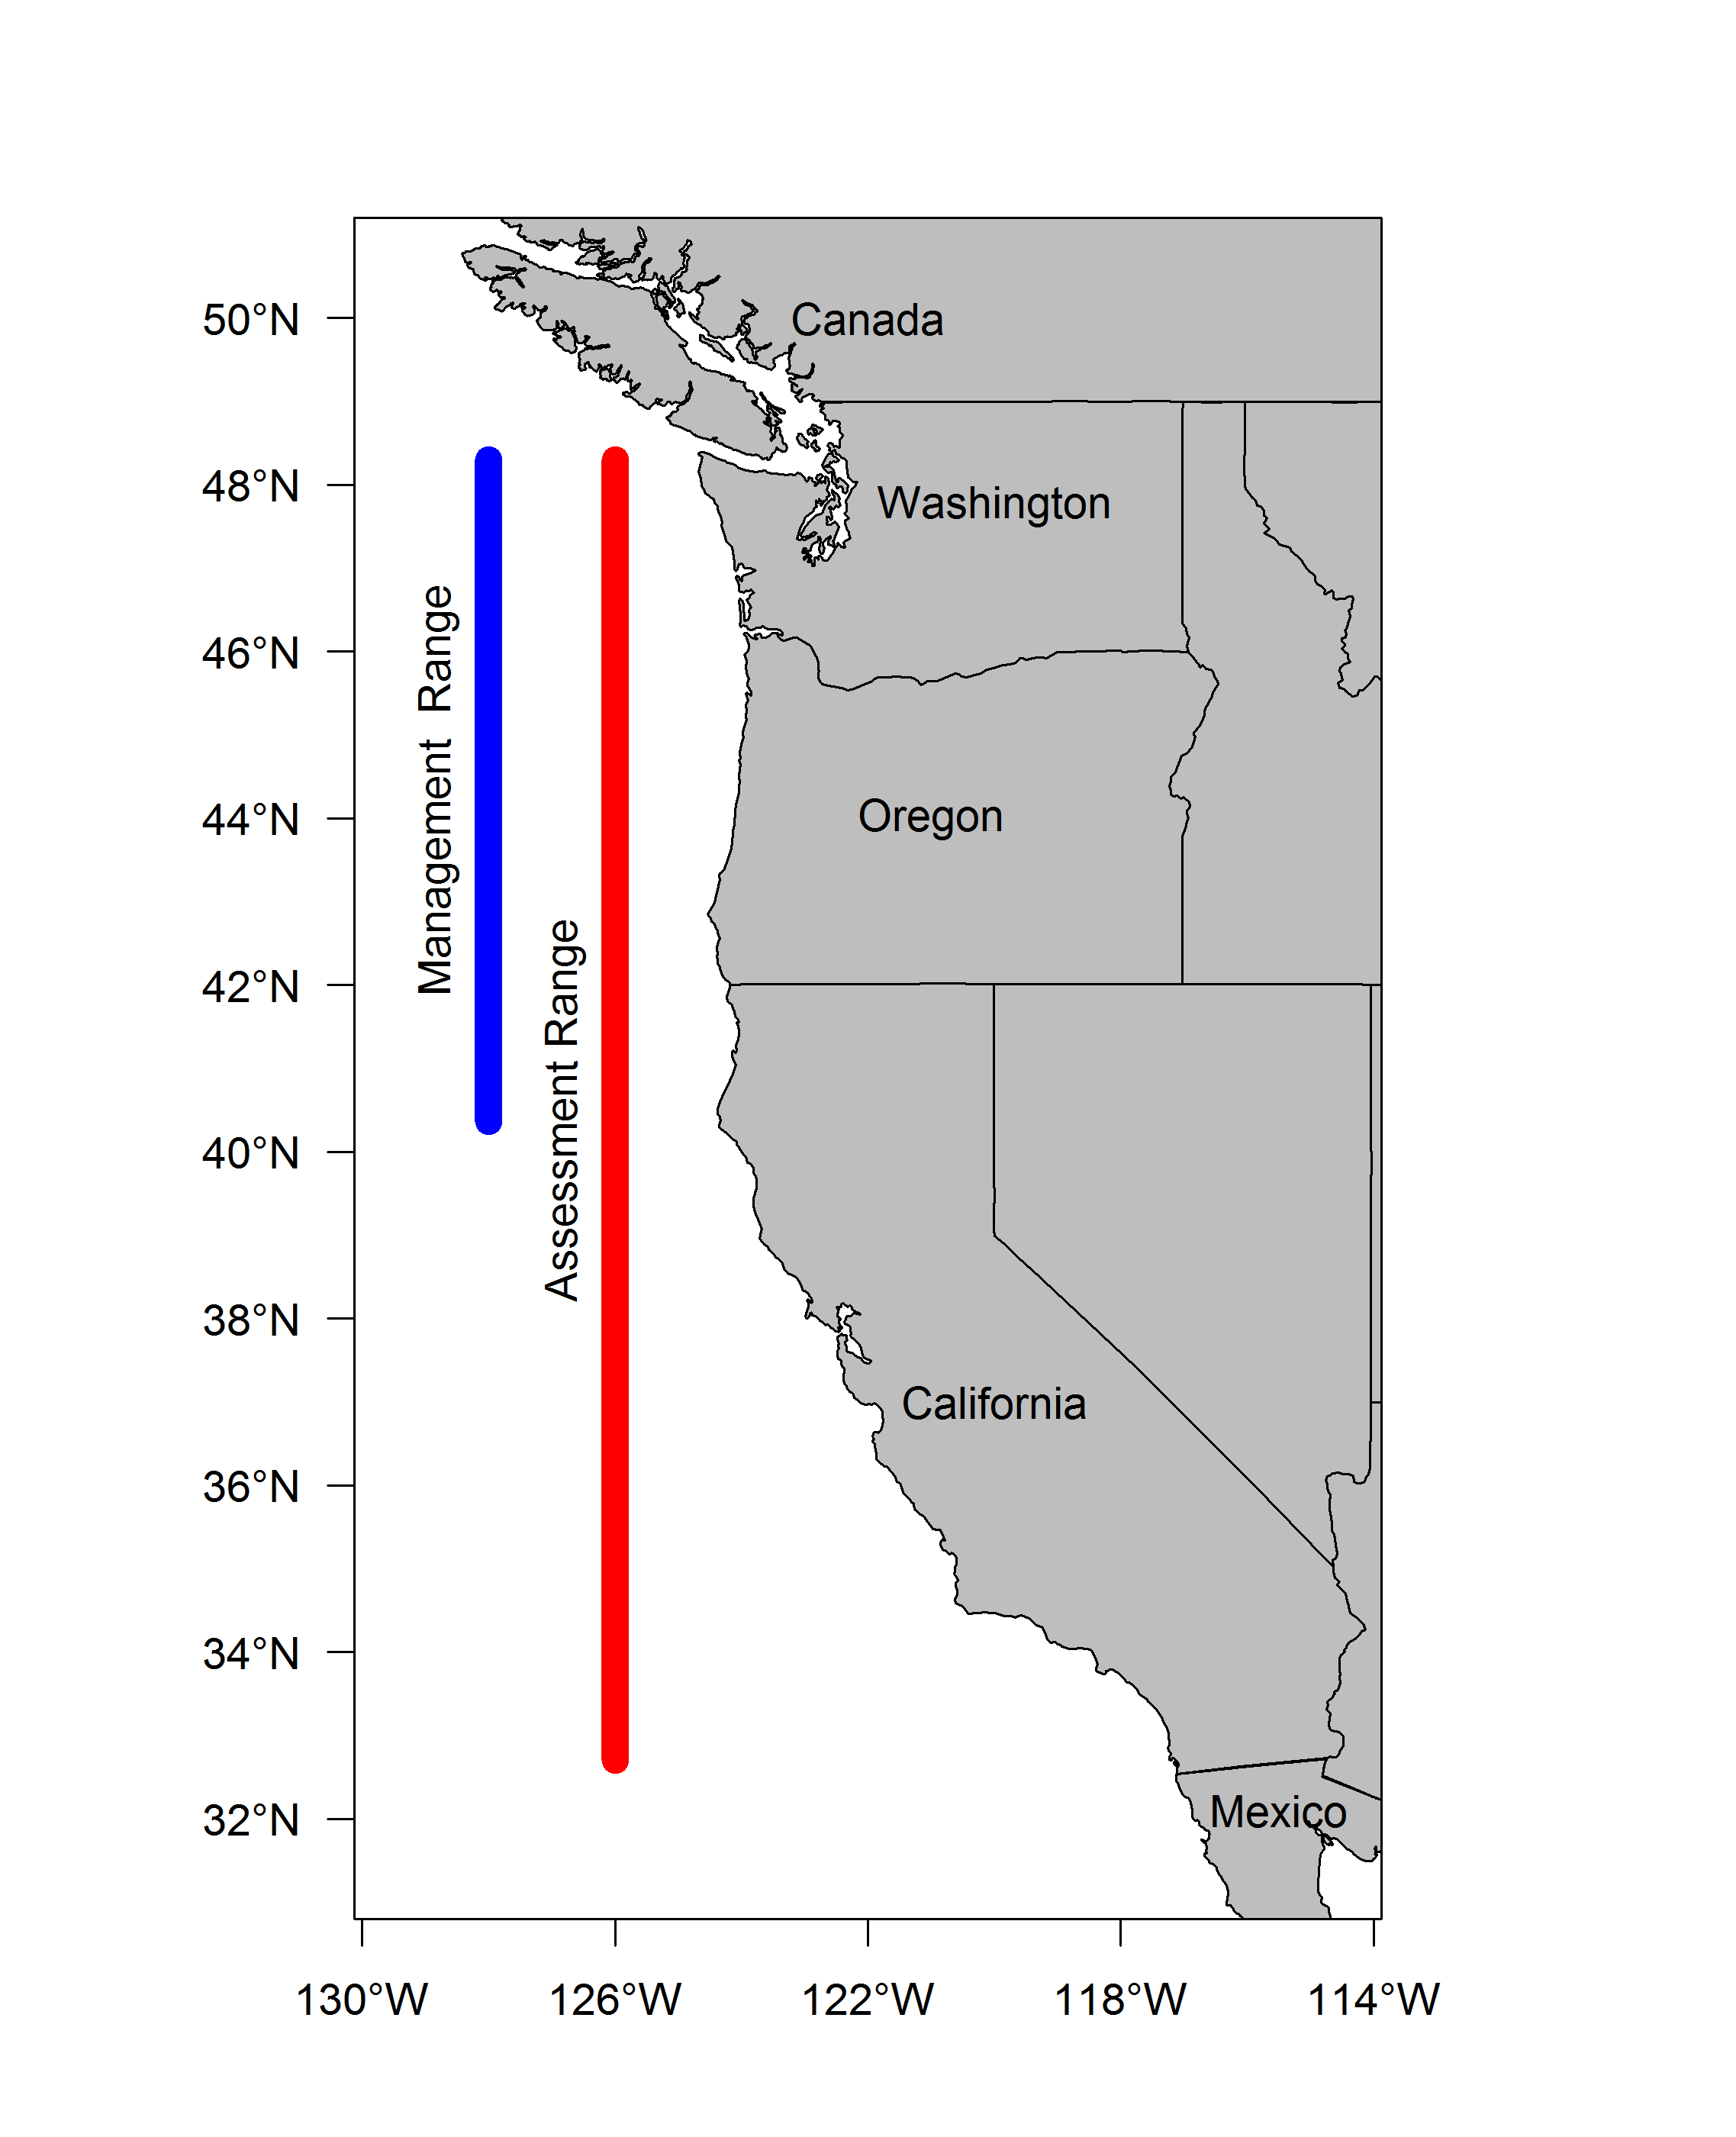
\includegraphics{assess_region_map.png}
\caption{Map depicting the boundaries for the base-case model.
\label{fig:assess_region_map}}
\end{figure}

\subsection{Slide with R created plot}\label{slide-with-r-created-plot}

\begin{Shaded}
\begin{Highlighting}[]
\KeywordTok{plot}\NormalTok{(pressure)}
\end{Highlighting}
\end{Shaded}

\includegraphics{Requets_Document_files/figure-latex/pressure-1.pdf}


\end{document}
